% !TeX root = ../thesis.tex
%*****************************************************************************************
%*********************************** Third Chapter ***************************************
%*****************************************************************************************

\chapter{On the Statistics of Macrospicules}
\label{ch:3} 

\section{Introduction}

Noticeable in \cref{sec:MS}, is the lack of recent statistical studies.
A statistical study would be particularly pertinent at this time, given that we now have a generation of advanced instruments with extensive catalogues of data.
It is now possible to re-examine the properties of macrospicules (MS) and improve the picture yielded in previous studies \emph{e.g.} \cite{Bohlin1975} and \cite{Dere89}. Furthermore, MS are chromospheric objects which project upwards into the transition region, hence understanding MS could enhance our knowledge of the region from the chromosphere up into the corona. We also need to confirm the features' place amongst the plethora of solar ejecta; jets, surges, rapid blue, or red, extensions, ordinary spicules to name a few \cite{Tsiropoula2012}.

The focus of this chapter is an observational discussion of what a macrospicule is; we present a set of characteristic spatial properties for the population of MS investigated as well as the evolution of the structures, and also an inquiry into whether the properties of the MS have any proxies to the solar cycle.

In order to analyse any potential relations over a solar cycle the sample of MS will be taken over a time span of many years. Hence, we will use the $30.4\ \textrm{nm}$ bandpass from the Atmospheric Imaging Assembly (AIA) camera on-board the Solar Dynamics Observatory (SDO) \cite{AIAspec}\, which has been in place and operating since June $2010$. As this was the epoch of the last solar minimum, we will take the sample through from this date until the end of $2012$. This range will capture the ramp from solar minimum to the period which is estimated to be close to the solar maximum. In order to gain a significant sample size we will take two samples of two hours for each month during this period.

\begin{figure}[h!]
	\centering
	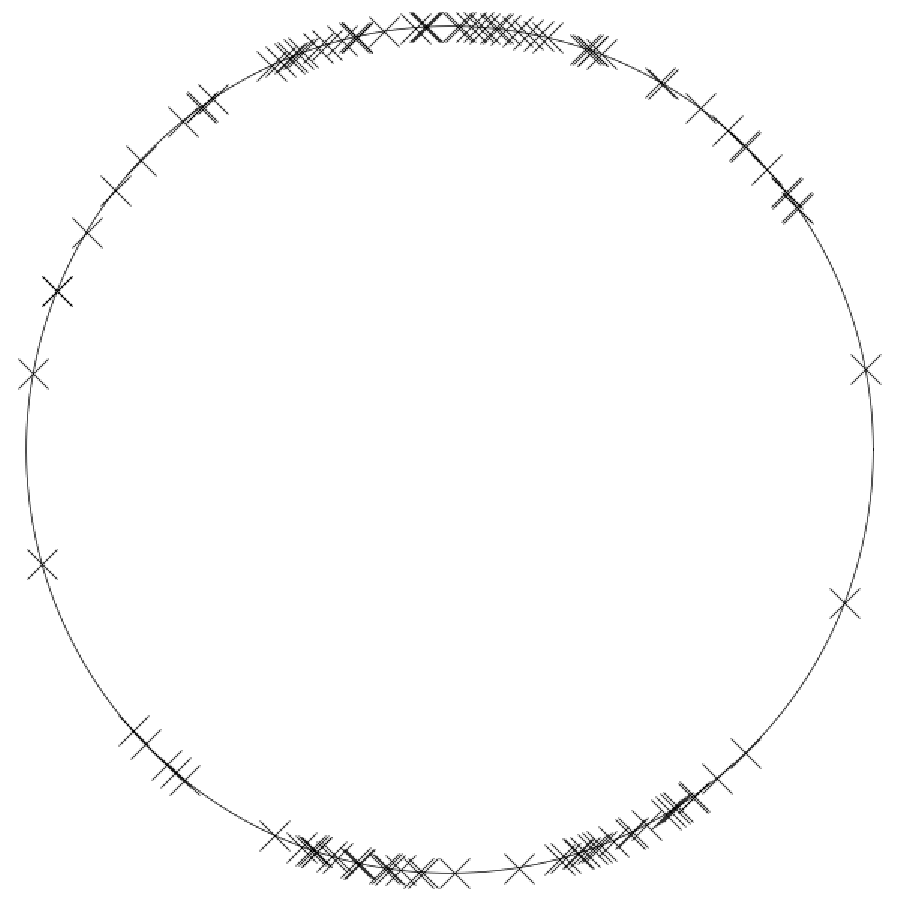
\includegraphics[scale=0.3]{Chapter3/Figs/polar_demo}
	\caption{\small The location of the samples of MS displayed at the limb, indicated by the crosses.}
	\label{fig:polar-sample}
\end{figure}


In \cref{sec:obs1} we present the relevant techniques used to take the measurements and the instrument utilised. \cref{sec:RandD1} presents the results of the study and discusses the consequences, specifically, with respect to the general spatial properties, followed by finding patterns over the sample time period and, then, a study of their evolution. \cref{sec:conc1} contains our conclusions. The work was published in \cite{Bennett2015}.


\section{Observations}
\label{sec:obs1}   
The AIA instrument on-board SDO delivers $4096 \times 4096$ pixel images with $0.6$ arcsec/pixel spatial resolution and a $12\ \textrm{s}$ cadence \cite{AIAspec}. Raw images were processed using SunPy [\cite{2015CS&D....8a4009S}], into a flattened-out limb such that the horizontal axis is the azimuthal angle and vertical is radius from the centre of the field of view. This allows a better measurement of the spatial properties of MS.


The MS were selected based on satisfying the following criteria: 
\begin{itemize}
	\item{ The evolution of the macrospicule is visible, \emph{i.e.} the extension from the chromospheric surface to its maximum height and consequent regression back to the limb. This excludes examples which appear to disintegrate at some point during its evolution or the retraction of which is not visible.}
	\item{The footpoint of the macrospicule was exactly on the limb, rather than inside of or behind the limb. Avoiding the MS which were too far inside the limb was aided by a limb indicating line, drawn based on information from the fits header files. Those events visibly crossing that line were not measured. It was harder to determine whether the MS were behind the limb, but we made our best effort to ensure that the measured MS were in the plane of sky, based on our inspection of the $30.4$ nm movies.}
	\item{The objects were no longer than $200\ \textrm{arcsec}$; there are values for maximum length quoted in \cite{Bohlin1975} and \cite{Dere89}, however, we would like to test the length limits of MS in order to more accurately define these phenomena. There is also a lower limit imposed upon us by the data itself. The so called `forest of spicules' at the solar limb prevents us from measuring any features with a maximum length of less then $5\ \textrm{Mm}$. We also call into question whether the features observed by those earlier authors were actually MS, there is certainly significant overlap in the lower percentiles of the population of spicules and MS.}
\end{itemize}


\begin{figure*}[t!]
	\centering
	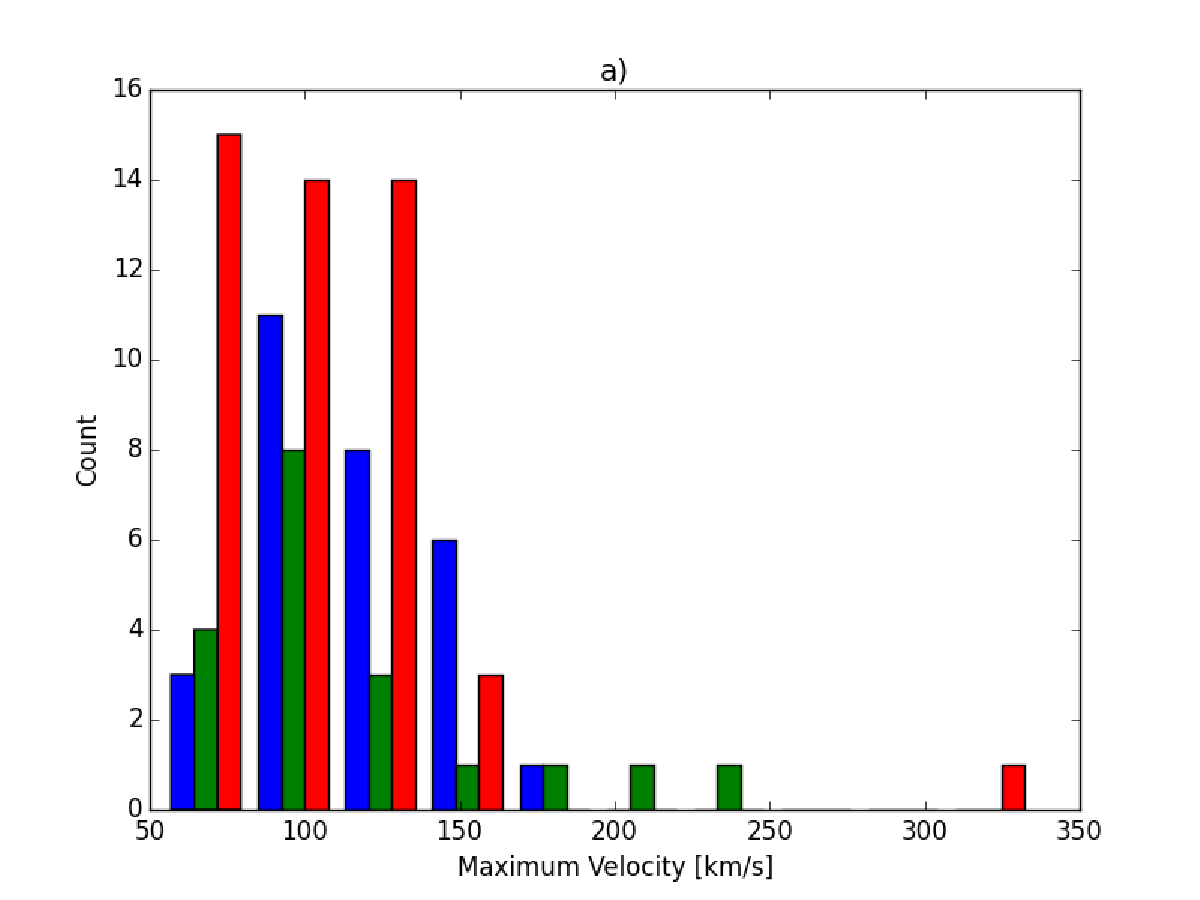
\includegraphics[width=0.49\textwidth, height=0.24\textheight]{Chapter3/Figs/vel_hist.pdf}
	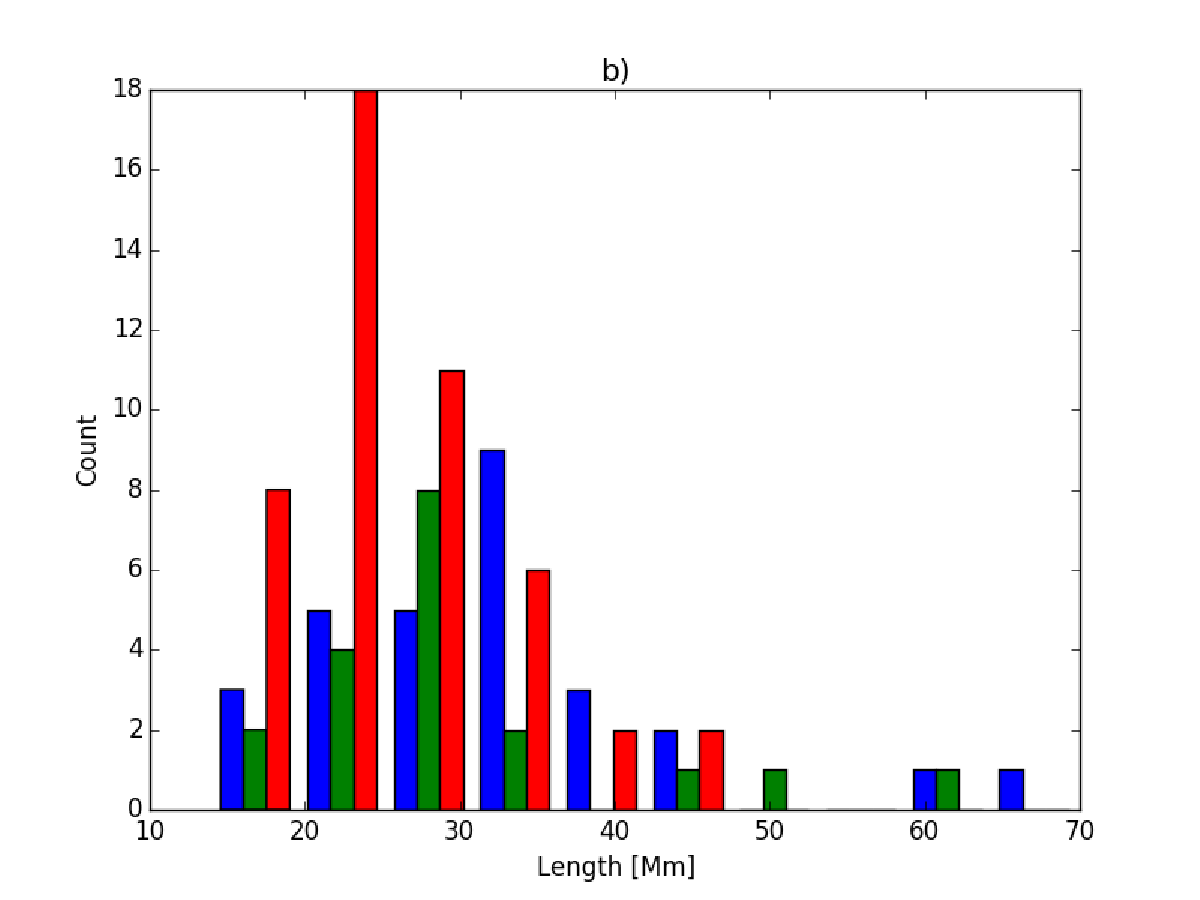
\includegraphics[width=0.49\textwidth, height=0.24\textheight]{Chapter3/Figs/len_hist.pdf}\\
	
	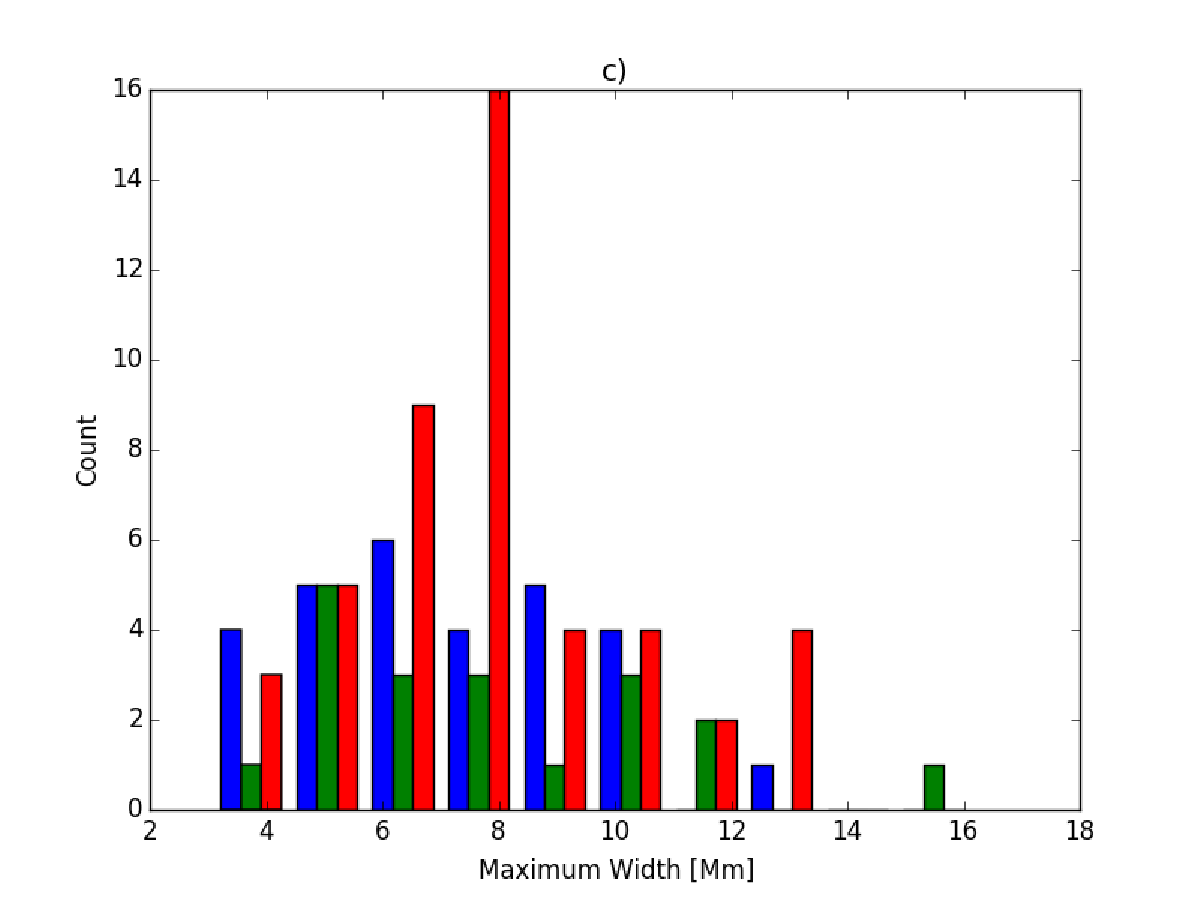
\includegraphics[width=0.49\textwidth, height=0.24\textheight]{Chapter3/Figs/width_hist.pdf}
	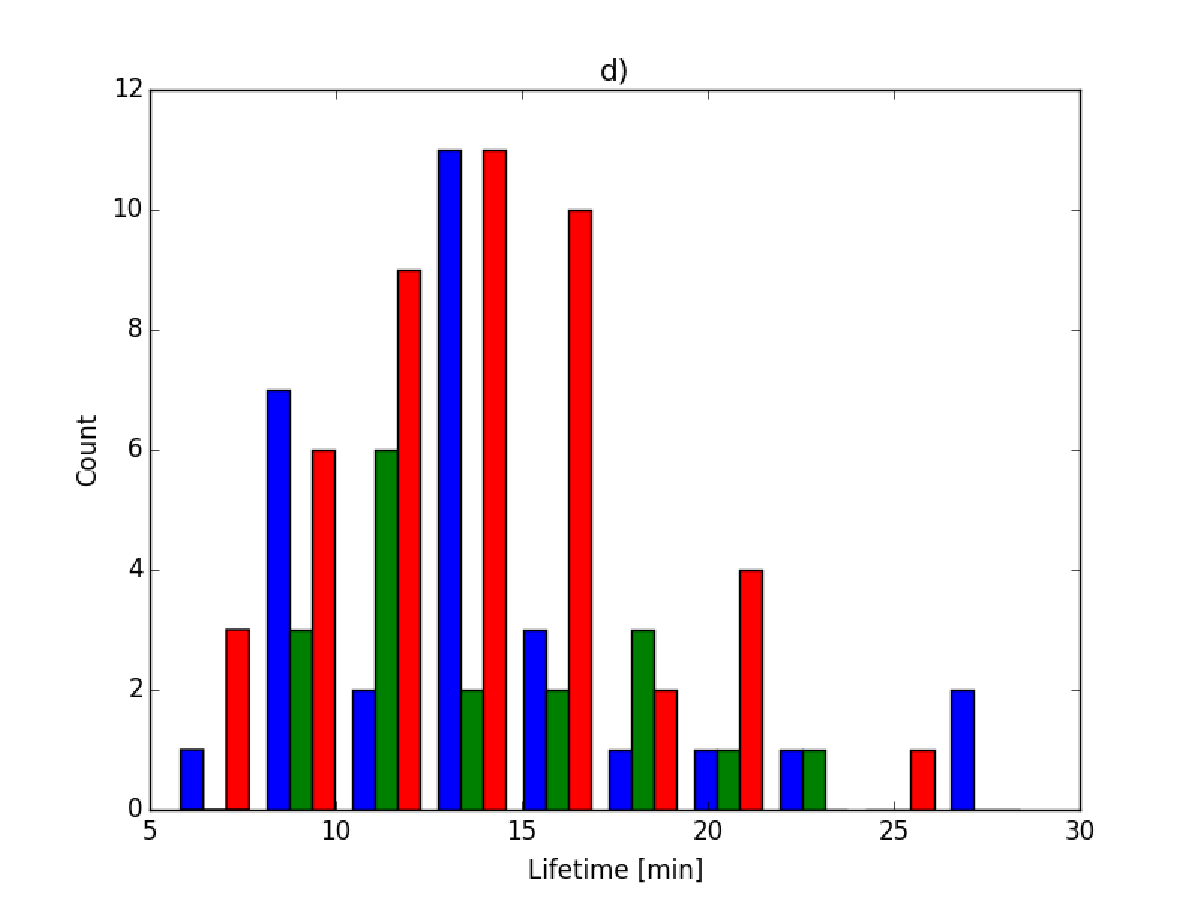
\includegraphics[width=0.49\textwidth, height=0.24\textheight]{Chapter3/Figs/lt_hist.pdf}	
	\caption{\small Figure taken from \cite{Bennett2015}. Histograms of properties of MS. In each bin counts from the 3 solar regions are displayed separately Blue indicates coronal hole MS, green represents coronal hole boundary MS and red are occurrences in the quiet Sun. a) top left. Histogram detailing the values of maximum velocity over the sample period. General grouping around the mean for all regions, $109.7\ \textrm{km/s}$, and an absence of clear distributions is evident, particularly in the quiet Sun, top left. b) top right. Detailing the maximum lengths, separate behaviour is found for all regions, quiet Sun displaying a distinctly lower peak, top right. c) bottom left. Maximum width of the MS, irregular distributions are clear with very little difference between the regions, bottom left. d) The lifetimes again show little difference in range, however MS at the coronal hole boundary have a slightly higher mean, bottom right.}
	\label{fig:basic-prop}
\end{figure*}


Each $30.4\ \textrm{nm}$ image was analysed separately and the length of the macrospicule in question is measured, defined here as the distance between the foot and tip of the macrospicule. We then took the mid point of the line between the foot and tip, and consequently used the mid point as a reference point for measuring the width. We used the bottom of the macrospicule brightening as $l_0$ and in situations where there was none, we used the lowest point at which plasma motion was initially observed. Using this method, we obtained information on the macrospicule with $12\ \textrm{s}$ cadence. Within the stated sample period we took $2$-hour samples on the $1$st and $15$th of each and every month.

Having undertaken the study, the distribution of the loci of macrospicule events measured along the solar limb is displayed in \cref{fig:polar-sample}. There are $101$ examples in this study. Note that there is some ambiguity in measuring spatial properties of features near the limb due to line-of-sight integration. However, without using data observing the MS from multiple directions, the best approximation is that MS are generated in the plane-of-sky, despite the potential uncertainties inherent in measuring at the limb.



\section{Results and Discussions}
\label{sec:RandD1}
Following the analysis of the MS as described above, the properties and, therefore, statistics for the sample of MS are found.
Of the sample we find that $30.5 \%$ of MS occurred in polar coronal holes, $20.0 \%$ occurred at the coronal hole boundaries and $49.5 \%$ were found in the quiet Sun.
The coronal hole boundary is defined loosely as the region where the coronal hole and quiet Sun meet. It is evident in the $30.4\ \textrm{nm}$ images that the coronal hole is significantly dimmer than the quiet Sun. 
Where these two regions meet, the quiet Sun and coronal hole structures combine over roughly $10$ Mm.
If a macrospicule is neither clearly in the quiet Sun or coronal hole in this region and within this region, it is defined as being in the coronal hole boundary.
Macrospicules generated near complex magnetic regions were not measured, due to the possibility of these regions influencing the measurement or of falsely identifying a feature as a macrospicule. Since active regions qualify as regions of complex magnetic field, MS forming in their proximity were excluded.


\subsection{General Properties}
%fixing all the references to figure
We begin with constructing the histograms for the individual properties, \emph{i.e.}, distribution of velocities, lengths, widths and lifetimes. Examining these general properties, we will consider each property in terms of the magnetic environments.

Beginning with the maximum velocities in \cref{fig:basic-prop}a, note the almost uniform distribution of MS found in the quiet Sun between $50$-$150\ \textrm{km/s}$ falling steeply after. The outlier in the $300$-$350\ \textrm{km/s}$ band is a value which may have errors. The respective range and mean values are, for the quiet Sun: $54.1$-$335.1\ \textrm{km/s}$ and $105.2\ \textrm{km/s}$, for coronal holes: $58.3$-$181.0\ \textrm{km/s}$ and $113.4\ \textrm{km/s}$, and for coronal hole boundaries: $66.8$-$236.0\ \textrm{km/s}$ and $114.5\ \textrm{km/s}$. These values are quoted with an error on each value of $\pm2.2\ \textrm{km/s}$.


We observe similar maximum velocity mean values for coronal holes and coronal hole boundaries while the quiet Sun has a lower average maximum velocity. This could imply different generation processes for MS in the coronal holes and at coronal hole boundaries, where reconnection is evident \cite{Patsourakos1999} and is a possible source for MS (see \cite{Heggland2009}). However, there is not enough evidence to conclude that MS are produced differently in other magnetic environments. Within the coronal hole it has been proposed that a collection of smaller spicules forms a macrospicule \cite{Scullion2009}, which would explain similar mean maximum velocities.

Where the maximum velocity occurs over the trajectory of the macrospicule is important, particularly for future modelling. We find that the maximum velocity of the macrospicule occurred within the first $19\%$ of the macrospicule's evolution in $68\%$ of cases.

\cref{fig:basic-prop}b shows the maximum lengths of all macrospicule instances. Investigation reveals ranges and means as follows, with errors of $\pm1.5\ \textrm{Mm}$; coronal hole lengths range of $17.3$-$69.8\ \textrm{Mm}$ with a mean $31.9\ \textrm{Mm}$, at coronal hole boundary the range is $16.1$-$60.2\ \textrm{Mm}$ with a mean $30.2\ \textrm{Mm}$ and for the quiet Sun the range is $14$-$45.3\ \textrm{Mm}$ with a mean of $25.4\ \textrm{Mm}$. 

We observe similar means and ranges for the lengths of the coronal hole and coronal hole boundary populations. This is unsurprising due to the open field nature of both regions allowing extension up the field lines. Whereas, in the quiet Sun, the mean value is $18\%$ less than those observed in the coronal hole/boundary. We draw attention to the narrower range in the quiet Sun as well. These values could be the consequence of the more complex magnetic field above the feature not allowing as much growth. 

From examining \cref{fig:basic-prop}c, detailing the maximum width of each macrospicule, it is evident that there are no distinct peaks in any of the populations in the coronal hole/boundary regions. After investigating the means, very similar values are revealed, $7.2$, $7.9$ and $7.8$ Mm for coronal holes, coronal hole boundaries and quiet Sun, respectively. The mean value for the quiet Sun coincides with the peak, but again, has no mathematically definable distribution. Of interest is the ratio between the width and length of MS, particularly useful in reference to modelling. Values found are; for coronal holes, $0.24$, for coronal hole boundaries, $0.26$ and for quiet Sun $0.32$, demonstrating that the width is small compared to the length of the macrospicule. Finally, it is evident that MS in the coronal hole/boundary regions have a lower ratio value than instances in the quiet Sun regions.

The lifetimes (\cref{fig:basic-prop}d) have a similar lack of difference between the populations seen in the width distribution. Ranges and means are as follows; for coronal hole $7.8$-$28.6\ \textrm{min}$ and mean $13.4\ \textrm{min}$, for coronal hole boundary $9.8$-$22.0\ \textrm{min}$ and mean $14.4\ \textrm{min}$, and for quiet Sun $5.6$-$30.6\ \textrm{min}$ and mean $13.6\ \textrm{min}$. The values obtained show similar ranges for coronal hole and quiet Sun instances but a smaller range for MS at the boundary. However we suspect that these are insignificant as the error in lifetime is $\pm1.1\ \textrm{min}$, implying that the means are similar for all three magnetic environments.

These values, found during the present analysis, are in-between the sets of values put forward by \cite{Bohlin1975} and \cite{Dere89}.

\subsection{Inclination} 
From previous studies it has been noted that MS have inherent inclination. \cite{Bohlin1975} noted that the further from the pole of the Sun the greater the inclination of the macrospicule. It is worth noting here that they did not in fact consider any MS outside of the coronal holes. 

We plotted the MS according to latitude and magnetic environment, \cref{fig:tilt-lat}. This graph shows the latitudes of each macrospicule instance against the degree of inclination; there are clear indicators where the coronal holes are. What is noticeable at this point is the fact that lower inclinations are associated with the ordinary coronal hole features but that MS occurring at the coronal hole boundary have a greater inclination, with no events which have a value lower than $15^{\circ}$. Quiet Sun events have an almost uniform distribution even appearing to occur in a coronal hole, but this is an artefact of the size of the coronal hole changing with the solar cycle and becoming very small as the Sun nears the solar maximum. 


\begin{figure}[t!]
	\centering
	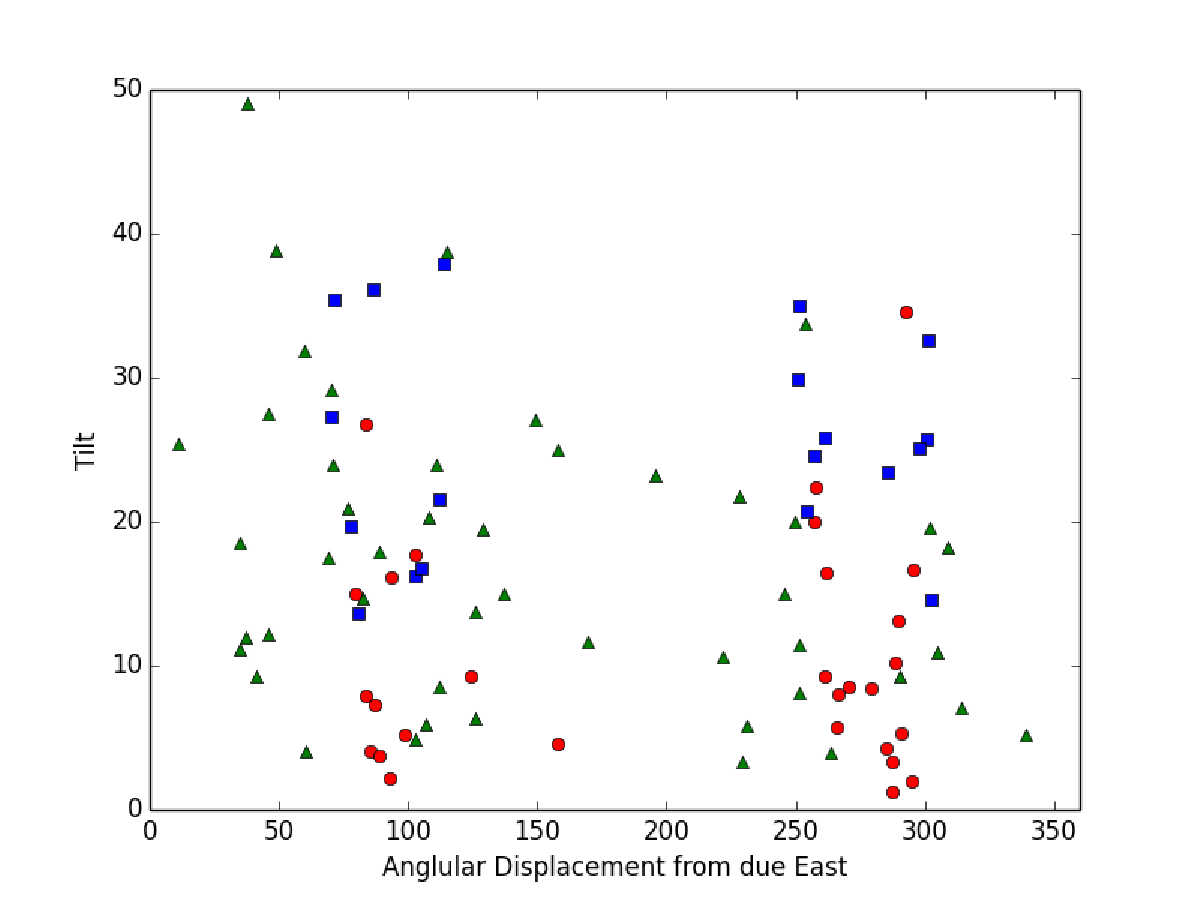
\includegraphics[width=0.5\columnwidth]{Chapter3/Figs/tilt_vs_lat.pdf}	
	\caption{\small Figure taken from \cite{Bennett2015}. Macrospicule events are plotted in terms of latitude and inclination. Inclination is defined here as the angle away from the normal to the limb of the Sun. The latitude is defined from due east and traces out anticlockwise. The red circles here are instances in the coronal hole, blue squares are at coronal hole boundaries and the green triangles are quiet Sun.}
	\label{fig:tilt-lat}
\end{figure}


\subsection{Relation between macrospicule properties}
It is worth investigating whether the properties, discussed earlier, have any empirical relation to each other. \cref{fig:prop-rel} shows the relationships between the maximum length, maximum velocity and lifetime of each macrospicule observation. Inspecting \cref{fig:prop-rel}a, reveals a clear correlation between the maximum length and the maximum velocity, as indicated by the least-squared regression, 

\begin{equation}
v = 61.3(1 + 0.28L),
\end{equation}

\noindent where $v$ [Mm/s] is velocity and $L$ [Mm] is the maximum length, the normal residual of which is $0.43$, indicating a significant fit. There is a particular exception in the top left of the plot which may have some errors and has altered the slope of the regression line quite distinctly.

There is a similar pattern to be reported in \cref{fig:prop-rel}b, where the lifetime and maximum length have been plotted against each other.

\begin{equation}
L = 10.39(1 + 0.12T),
\end{equation}

\noindent where $L$ length in Mm and $T$ is the lifetime in min and normal residual value $0.66$. This value is small compared the average maximum length, therefore the fit is reliable. Again, there are a few extreme instances which may not be a part of the overall macrospicule population, such as the instance in the bottom right with a short maximum length but long lifetime. 

Lastly, \cref{fig:prop-rel}c, shows the relationship between the maximum velocity and the lifetime of MS, defined,

\begin{equation}
v = 88.9(1 + 0.016T).
\end{equation}

Incongruously, relationship between the maximum velocity and the lifetime of the MS is unclear. A shallow trend is apparent in the scaling factor, $0.016$, which is inconclusive as to whether a relationship exists between the two properties, however it is unlikely.

\begin{figure}[h!]
	\centering
	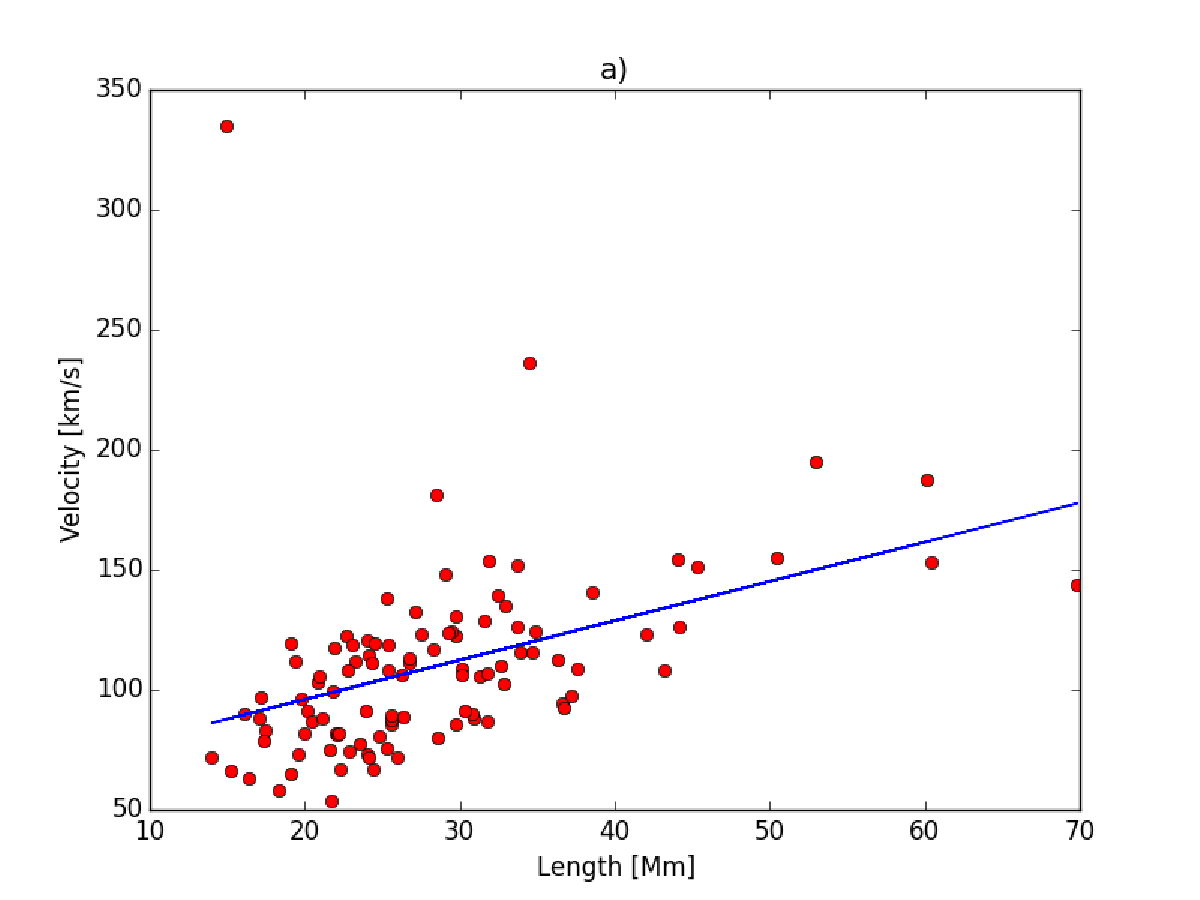
\includegraphics[width=0.4\textwidth]{Chapter3/Figs/length_max_vs.pdf}
	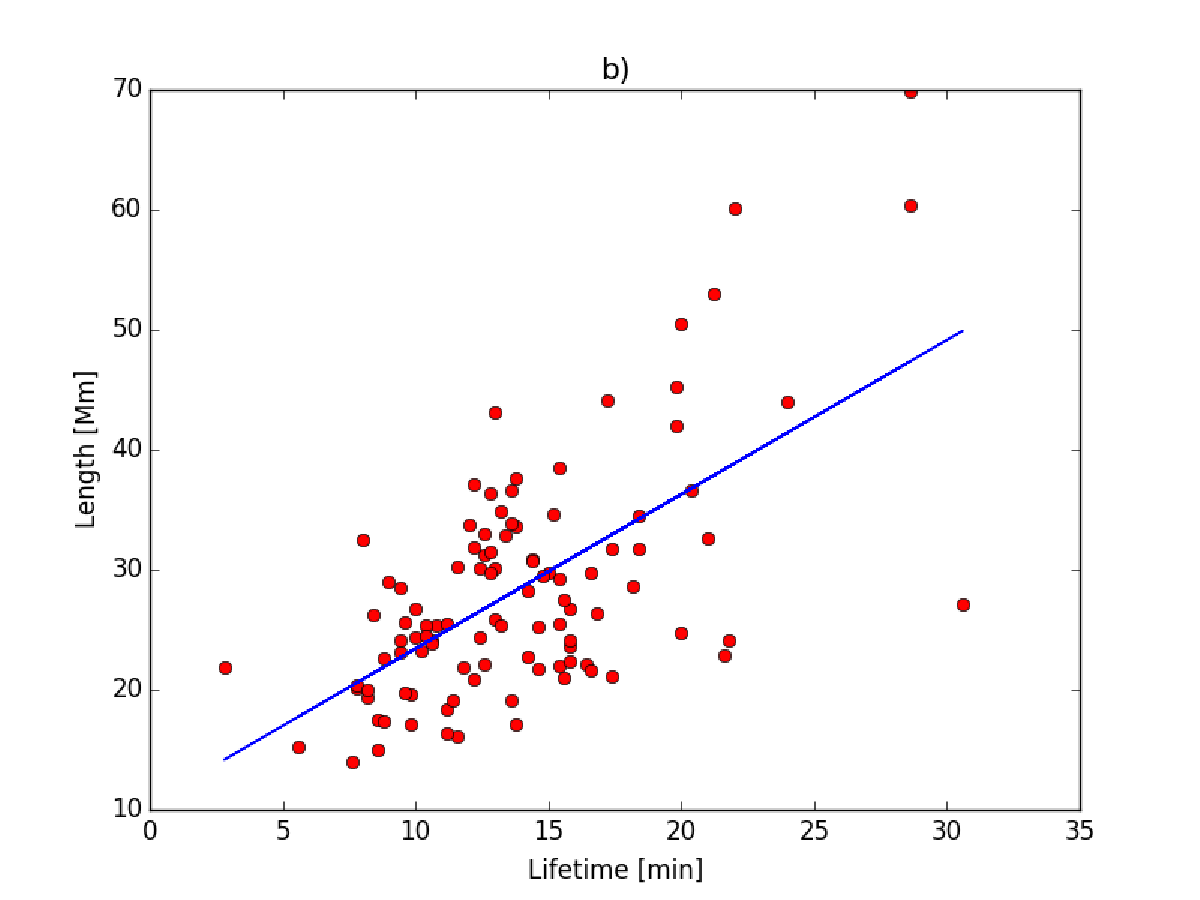
\includegraphics[width=0.4\textwidth]{Chapter3/Figs/lifetime_vs_length.pdf}
	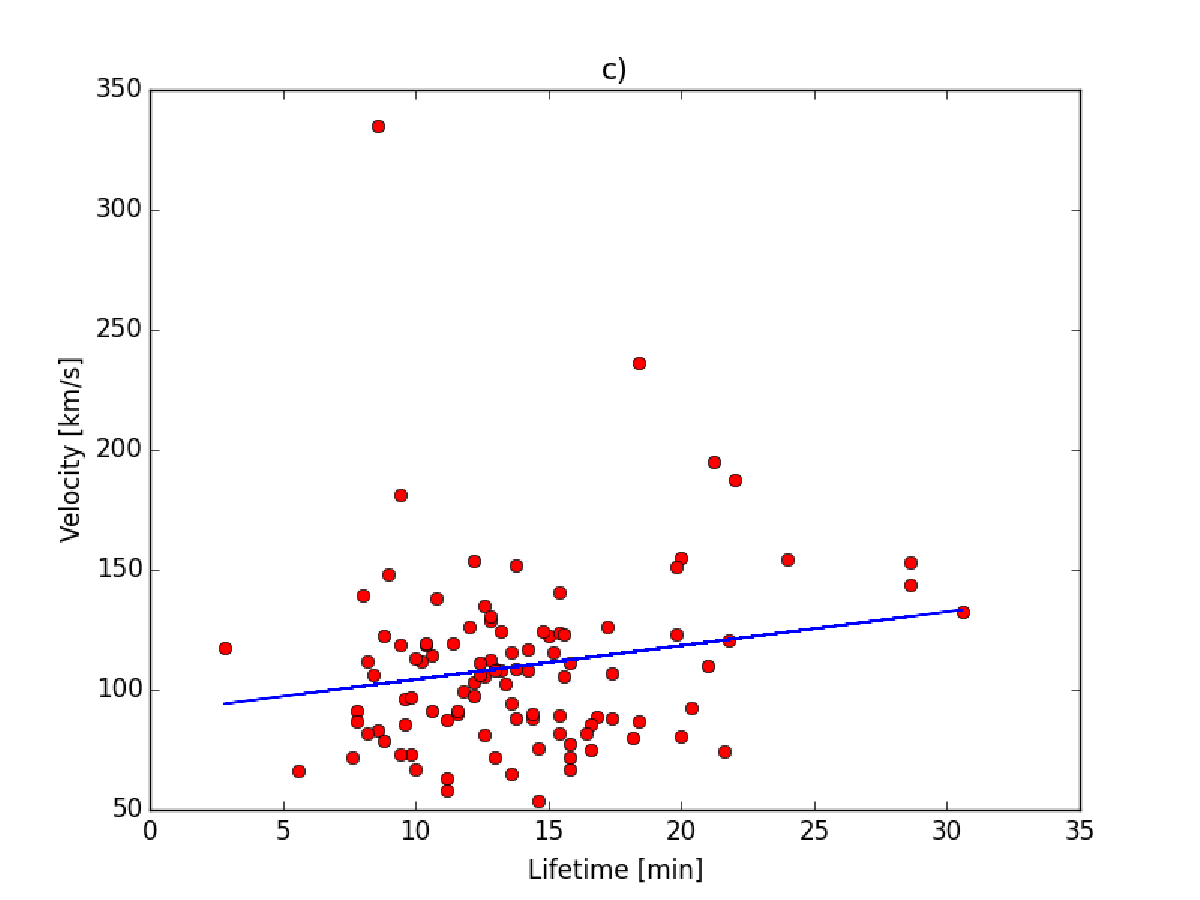
\includegraphics[width=0.4\textwidth]{Chapter3/Figs/velocity_vs_lt.pdf}
	\caption{\small Taken from \cite{Bennett2015} Properties of MS features plotted with respect to each other. a) Top: The max length against the max velocity for each individual instance. The least-squares fit shows a distinct correlation. b) Middle: The lifetime vs max length graph shows a similar degree of correlation between these two properties, middle. c) Bottom: In the case of max velocity and lifetime, there is no such relation, as is indicated by the least squares fit and scaling equation (below). Error bars associated with the least squares fit are omitted as the standard error is small compared to the range of values.}
	\label{fig:prop-rel}	
\end{figure}


\subsection{How the macrospicule general properties change over the sample period}
The investigated sample period is a proxy for the process by which the Sun's activity increases from solar minimum in $2010$ up to solar maximum at the end of $2012$. Therefore, examining the macrospicule properties over the sample period is a worthy exercise and may give insight into the cause of MS. \cref{fig:sol-cyc-rels} illustrates how the general properties alter over the sample time period. Examining first the maximum length, \cref{fig:sol-cyc-rels}a, shows a relationship over the entire sample period, with some instances where the maximum length values do not appear to be part of the overall population. 

However, these examples, which are over $50\ \textrm{Mm}$, are not necessarily too extreme to be classed as MS. Upon visual examination of the five most extreme examples there are no discernible differences in the four instances between $50\ \textrm{Mm}$ and $60\ \textrm{Mm}$ in height. The most extreme example, $69.8\ \textrm{Mm}$, does appear separate from the population. It is wider than average and the structure is less defined and more fractious. This can be removed from the sample. The mathematical relation of the fitted line, using least squares, reflects the general trend upwards over the sample time period, 

\begin{equation}
L = 24.9(1 + 0.11t),
\end{equation}

\noindent where $L$ is the maximum length of a macrospicule and $t$ is the point in time. The gradient value is small, but is a result of the long period over which the sample has been taken.

Studying the lifetime property of the MS over the solar cycle in \cref{fig:sol-cyc-rels}b we, again, notice an increase over the sample-time period, though the gradient is not as steep as that of the fit for the maximum lengths, 

\begin{equation}
T = 12.7(1 + 0.074t),
\end{equation}

\noindent where $T$ [min] is the lifetime of a macrospicule and $t$ is the time [years]. There seems to be a general population close to the fit with only a few extreme examples, e.g. one below the general population and 3 above $25\ \textrm{min}$. We closely examined the extreme examples in this case as well. Only the macrospicule with the longest lifetime showed any particular differentiation from the rest of the population. Greater width is observed alongside apparent separate structures within the macrospicule, therefore this instance is eliminated from the study.

The most interesting result here is that when inspecting the maximum velocity over the sample period, see \cref{fig:sol-cyc-rels}c. We notice that the maximum velocity changes very little, the magnitude of the gradient is indicative of a small decline, 

\begin{equation}
V = 113.03(1 - 0.025t),
\end{equation}

\noindent where $V$ is the maximum velocity in Mm/s. Given that we found that in \cref{fig:sol-cyc-rels}c, the maximum length and maximum velocity are related, one would naturally expect the maximum velocity to show a similar behaviour over the sample time period. Again, we visually examined the extreme examples eliminated two instances, a maximum velocity of $335.9\ \textrm{km/s}$ was clearly an error in measurement and so has been removed and the second is not clearly defined and may have suffered from limb effects. (All extreme examples are included in the graphs here, but however are excluded from our final statements.)

\begin{figure}[h]
	\centering
	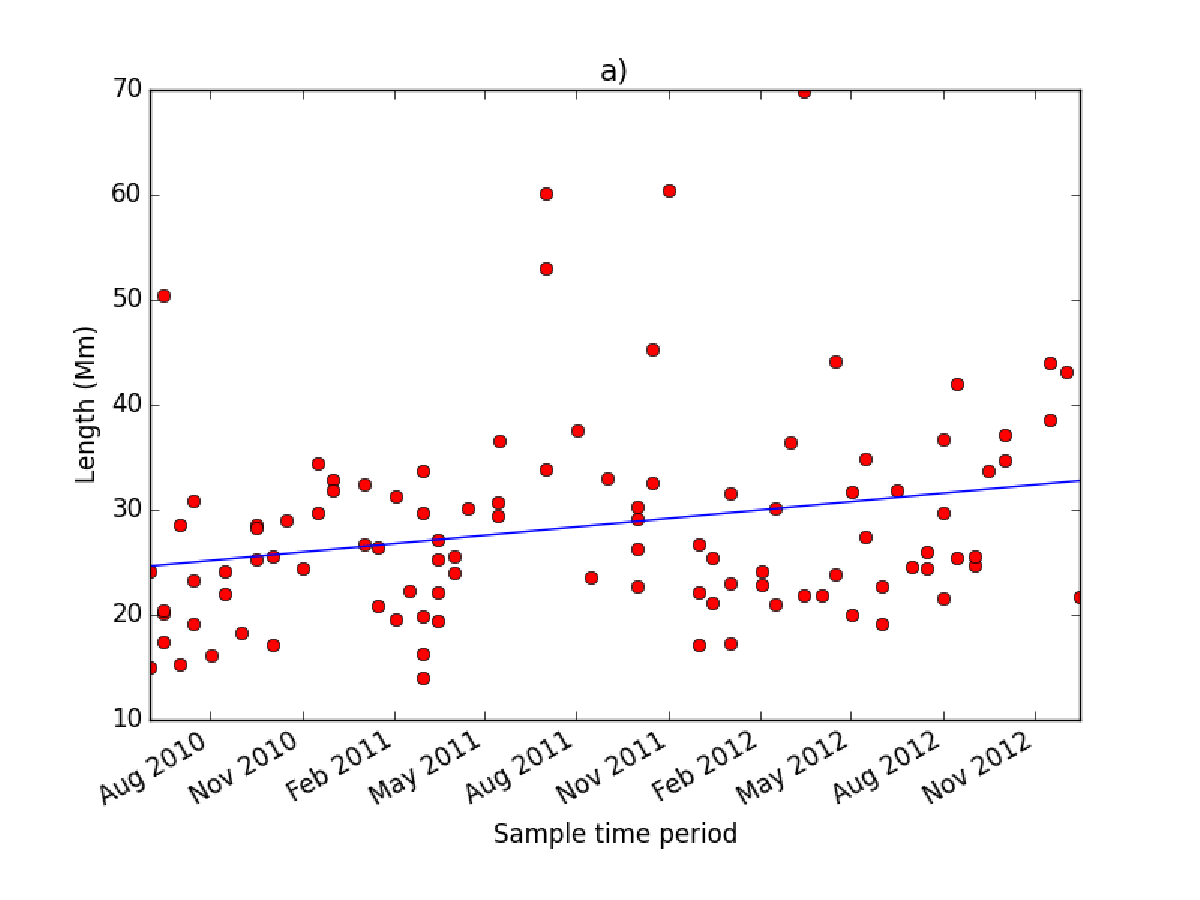
\includegraphics[width=0.4\columnwidth]{Chapter3/Figs/length_vs_solarcycle.pdf}
	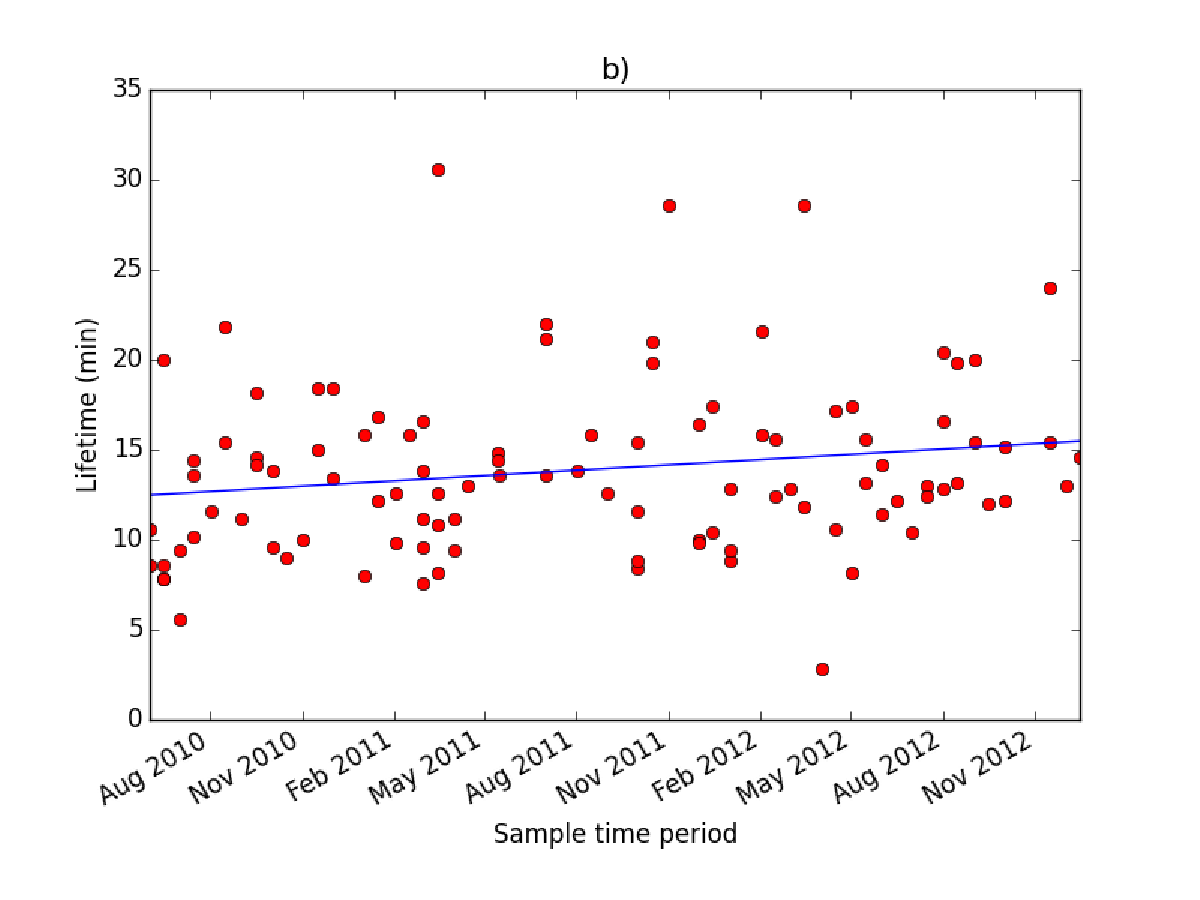
\includegraphics[width=0.4\columnwidth]{Chapter3/Figs/life_vs_solarcycle.pdf}
	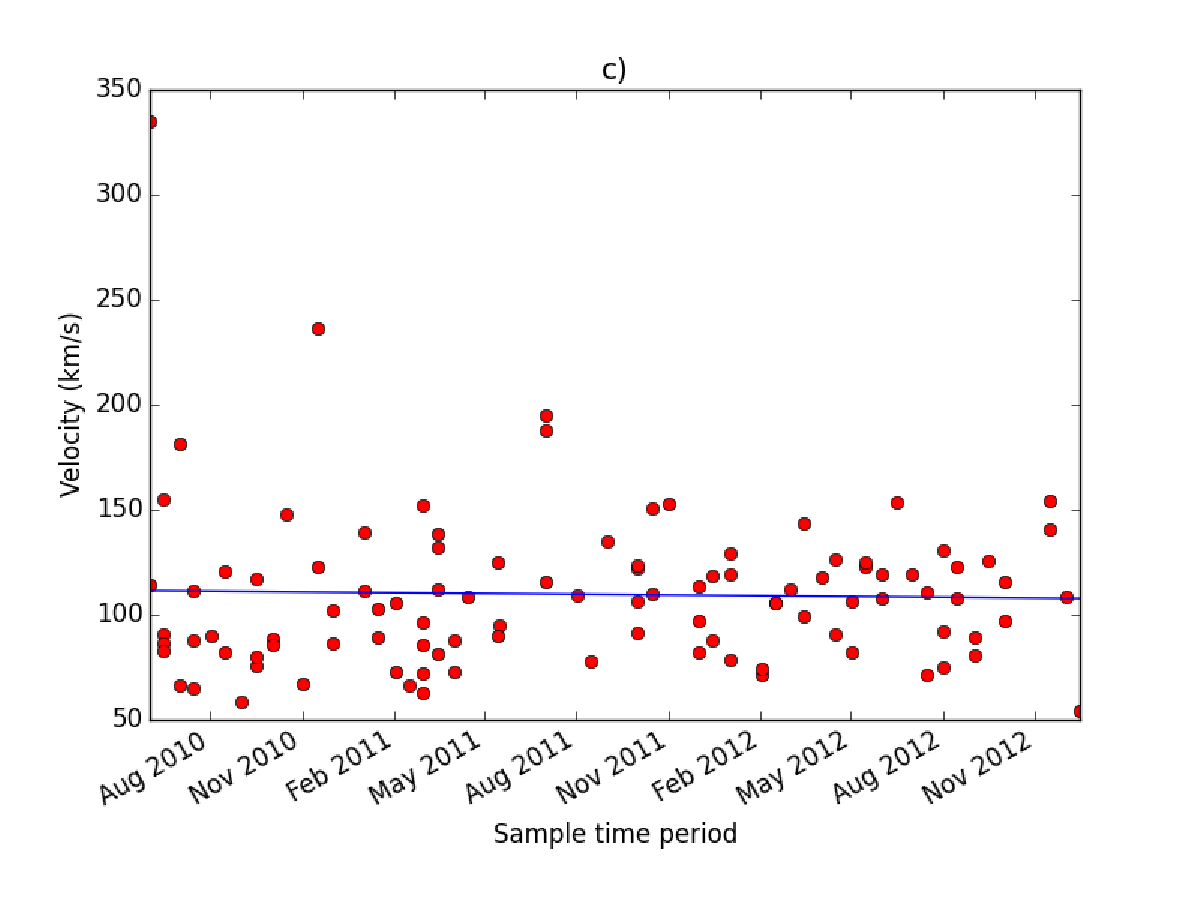
\includegraphics[width=0.4\columnwidth]{Chapter3/Figs/velocity_vs_solarcycle.pdf}
	\caption{\small Figure from \cite{Bennett2015}. Macrospicule properties over the sample time period. Notice that the graphs for maximum length and lifetimes, a) top and b) middle, respectively, have general trends with a positive gradient over the sample time period, while the maximum velocity graph, (c, bottom panel) has none of the same trends apparent in the others.}
	\label{fig:sol-cyc-rels}
\end{figure}


\subsection{Ballistics}
How the features behave over their life-span is important in terms of possible generation mechanisms, and how they may interact with the transition region. SDO has limited spectral data as AIA is an imager. Therefore, readings are limited to spatial measurements. One interesting question is whether MS have a ballistic nature such that upon reaching their highest point they would then fall back only under the influence of the Sun's gravity. The question is of importance due to the nature of ordinary spicules typically located at granular lanes.

Current research proposes two varieties of spicules, type-1 and type-2, \cite{Pereira2012}, but \cite{Zhang2012} debates this point, and finds no such population split. We believe that names of physical phenomena should be based on the underlying physics, not arbitrary behaviour. Type-1 spicules are potentially driven by \emph{p}-mode global oscillations, and spicules typically have lifetimes of $4$ - $10\ \textrm{mins}$ and heights $7$ - $10\ \textrm{mins}$ \cite{DePointeu2004}.

Type-2 spicules are most likely reconnection events, which might explain their high velocities, similar lengths to type-1 and typically observed with much shorter lifetimes, $10$ - $150\ \textrm{s}$, \cite{Isobe2008}. Type-2 spicules are observed not to fall back to the solar surface, however, there is debate as to whether these features are physical, or an artefact of observation \cite{Tsiropoula2012}, \cite{Sekse2013} or finally whether their regression is observed in a different wavelength \cite{Pereira2014}.

The question becomes: are these MS giant versions of \emph{p}-mode spicules, or are they blown-up manifestations of reconnection spicules. Alternatively, are they related to these ejecta at all? In order to answer these questions, one needs to understand what the underlying driving mechanism for Type-1 and Type-2 spicule. Consequently, one needs to find signatures of driver(s) in the formation of MS. An interesting alternative suggestion for generation of MS is a model where multiple spicules form a macrospicule \cite{Xia2005}.

The final case is that MS and spicules are not related in their formation at all. \cite{Shibata1992} proposed a jet formation model which has become known as the `Inverted Y' jet model which occurs on much larger scales than spicules. Using Yohkoh's soft X-Ray Telescope (SXT), they highlighted the X-Ray jets had lengths in the $5$-$40\ \textrm{Mm}$ and velocities in the order $30$-$300\ \textrm{km/s}$, notably, similar to the values we have quoted above. This fits in with the observations of \cite{Moore1977} of X-Ray bright points coinciding with H$\alpha$ MS, (also supposed in \cite{Kamio2010}). Another model presented by \cite{Jiang2007} proposes magnetic flux emergence as a source for H$\alpha$ and EUV jets. They find lengths similar to those discovered as well, $4$-$22\ \textrm{Mm}$ with a lifetime range of $10$-$34\ \textrm{mins}$ (including cool and hot aspects of the jet). Both values are also comparable to those we observe in this study.

Given this, one might expect that there is a consensus that these are the same objects observed in different wavelengths, however, this is not the case. \cite{Moore2010} highlight a dichotomy in solar coronal jets, certainly between the standard jets \cite{Shibata1992} and blowout model for jet formation which the authors described. The authors concluded that the blowout jet model results in Helium $30.4\ \textrm{nm}$ MS forming from base arches of the order $10\ \textrm{Mm}$ in width. If we assume that MS observed in H$\alpha$ and Helium $30.4\ \textrm{nm}$ are the same feature as supposed by \cite{LaBonte79} and implied by \cite{Parenti2002}, then is it reasonable to propose that the blowout jet mechanism also drives EUV MS.

Examining \cref{fig:ballistics} there are two particular trends to note. The first is shown in \cref{fig:ballistics}a, where the times for the regression back down to the solar limb were taken from the observational values, blue point in the figure, and times calculated using basic gravitational laws, assuming point mass and free-fall under uniform gravitational acceleration from the tip of the macrospicule, are in red. 

We observe similar times for regression back to the limb for the estimates and the recorded times. Clearly there is a greater variance in the measured values compared to the estimates, but this is to be expected. The mean time for the tip to recede back to the limb is $7.5$ min estimated and $6.6\ \textrm{min}$ recorded, with the similar values indicating that gravity is the dominating force behind their fall. The difference between the two sides of the evolution is $6.6\%$ of the average overall lifetime, which is likely not large enough to be significant. 

Let us now make a brief comparison of this behaviour described by the current literature. Recent studies have found that the time taken for a jet to fall back to the solar surface is greater than expected from a ballistic model. \cite{Nishizuka2011} have found that chromospheric jets (small jets, $1$-$4\ \textrm{Mm}$ in length with a magnetic anemone base) share similar motions with the shock-acceleration model demonstrated in \cite{ShibataSuematsu1982}, notably, slower than a ballistic model. \cite{Moschou2013} also find velocities lower than those under a ballistic model, however, the features highlighted here are much larger, measuring $100$-$190\ \textrm{Mm}$ in length, than MS. \cite{Feng2012} demonstrate that kinematic motions of the particles in jets follow ballistic trajectories. Therefore it is possible that in MS the plasma-beta is high, and the entire feature follows the ballistic nature of the gas particles. Otherwise, the observed motion may be due to the surrounding magnetic environment. Macrospicules examined here were deliberately chosen in locations where there was a lack of complicated magnetic environment, hence would be allowed to evolve on their own.



\Cref{fig:ballistics}b, demonstrates the change in width either side of the greatest extent of the macrospicule as a percentage. We find that after the peak of the macrospicule, the width actually decreases on average with MS being $20\%$ smaller. This could be due to plasma flowing down magnetic field lines causing a thinning within the macrospicule. This could delay the collapse of the macrospicule and cause the slightly longer recorded times as opposed to the estimated times.       

\begin{figure}[h!]
	\centering
	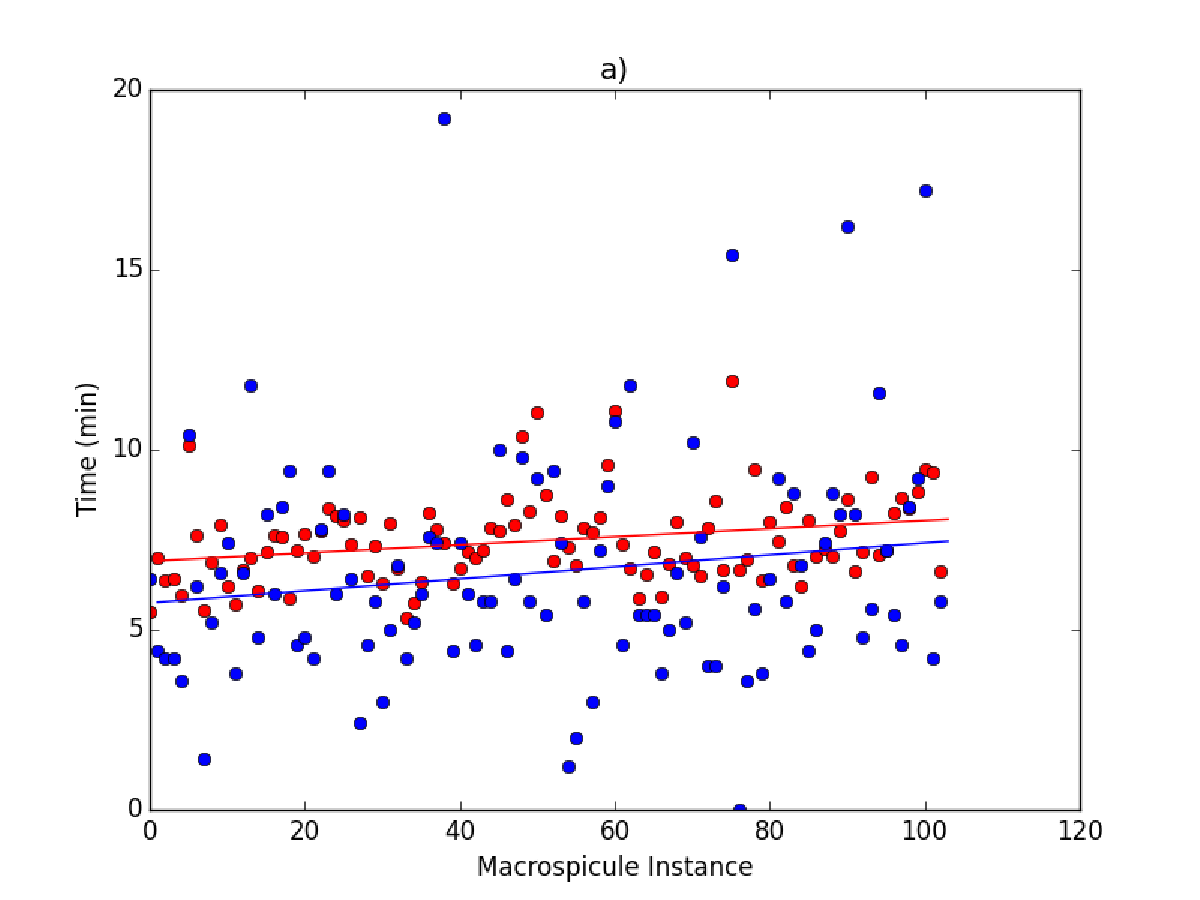
\includegraphics[width=0.48\textwidth]{Chapter3/Figs/times_falling.pdf}
	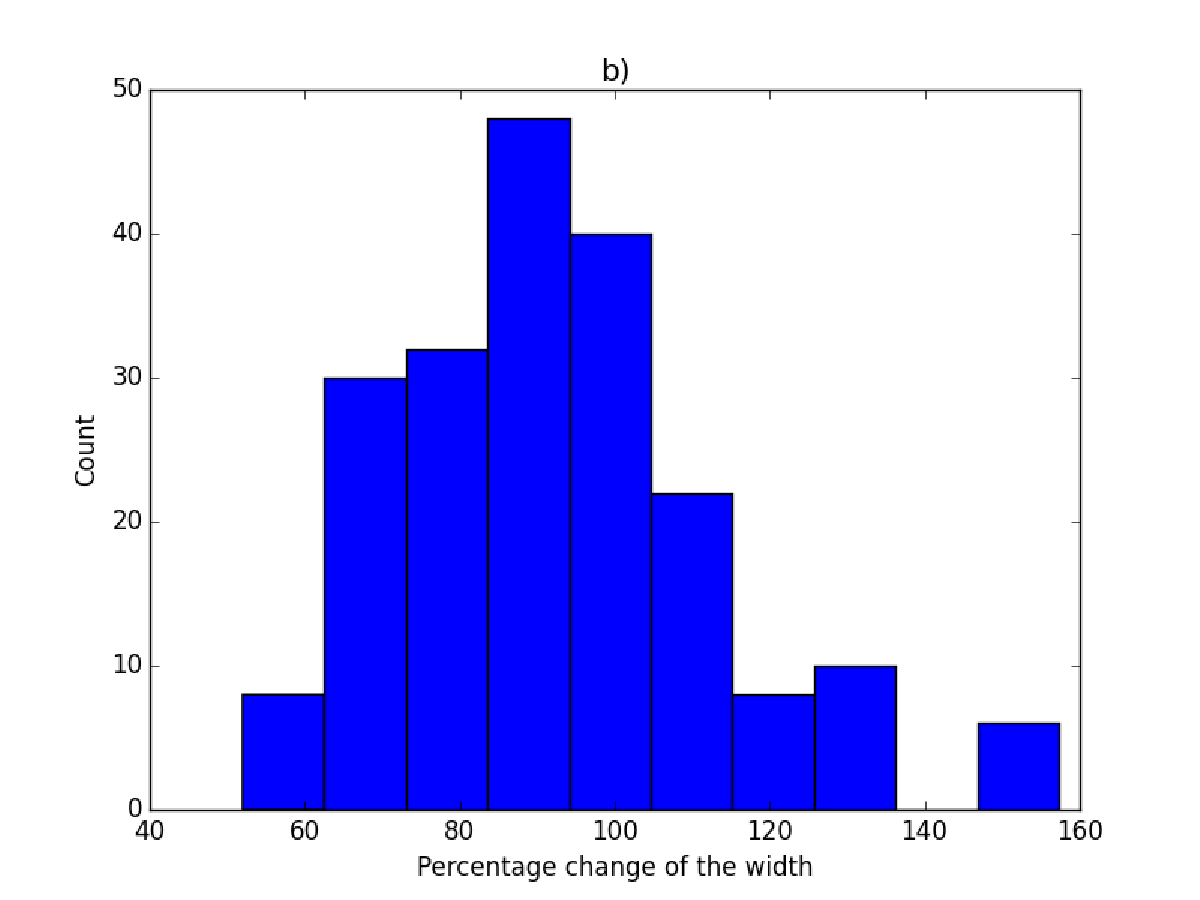
\includegraphics[width=0.48\textwidth]{Chapter3/Figs/width_percent.pdf}
	
	\caption{\small Estimated times for a point mass falling from the apex of the macrospicule trajectories, a) top, for the macrospicule are red, while the times taken from the data are blue points, top panel. There is little deviation from ballistic model evident in the MS measured times. b), bottom, the percentage change in width. The widths are taken before and after the peak of the length-time plot as a percentage change. The width is smaller, on average, after the peak.}
	\label{fig:ballistics}
\end{figure}

\begin{figure}[h!]
	\centering
	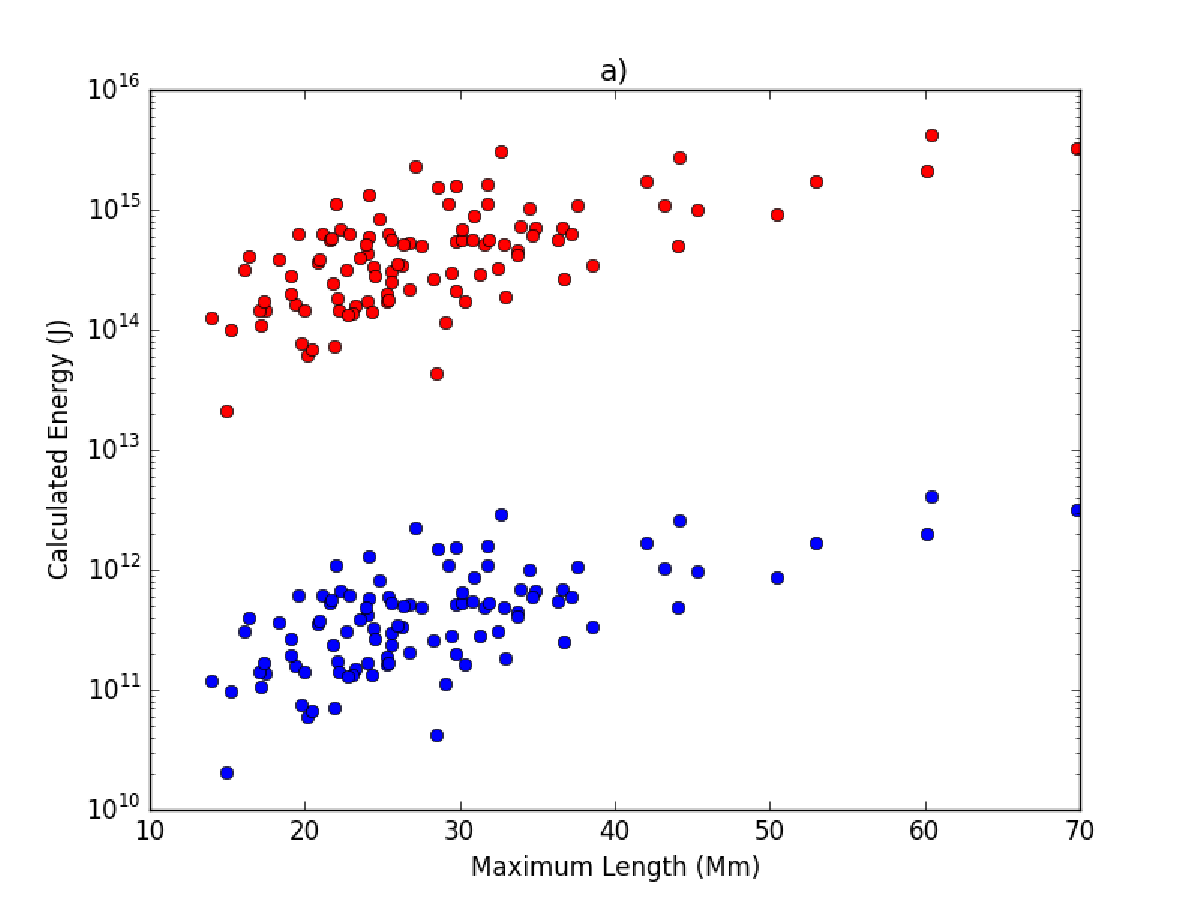
\includegraphics[width=0.48\textwidth]{Chapter3/Figs/diff_rho0.pdf}
	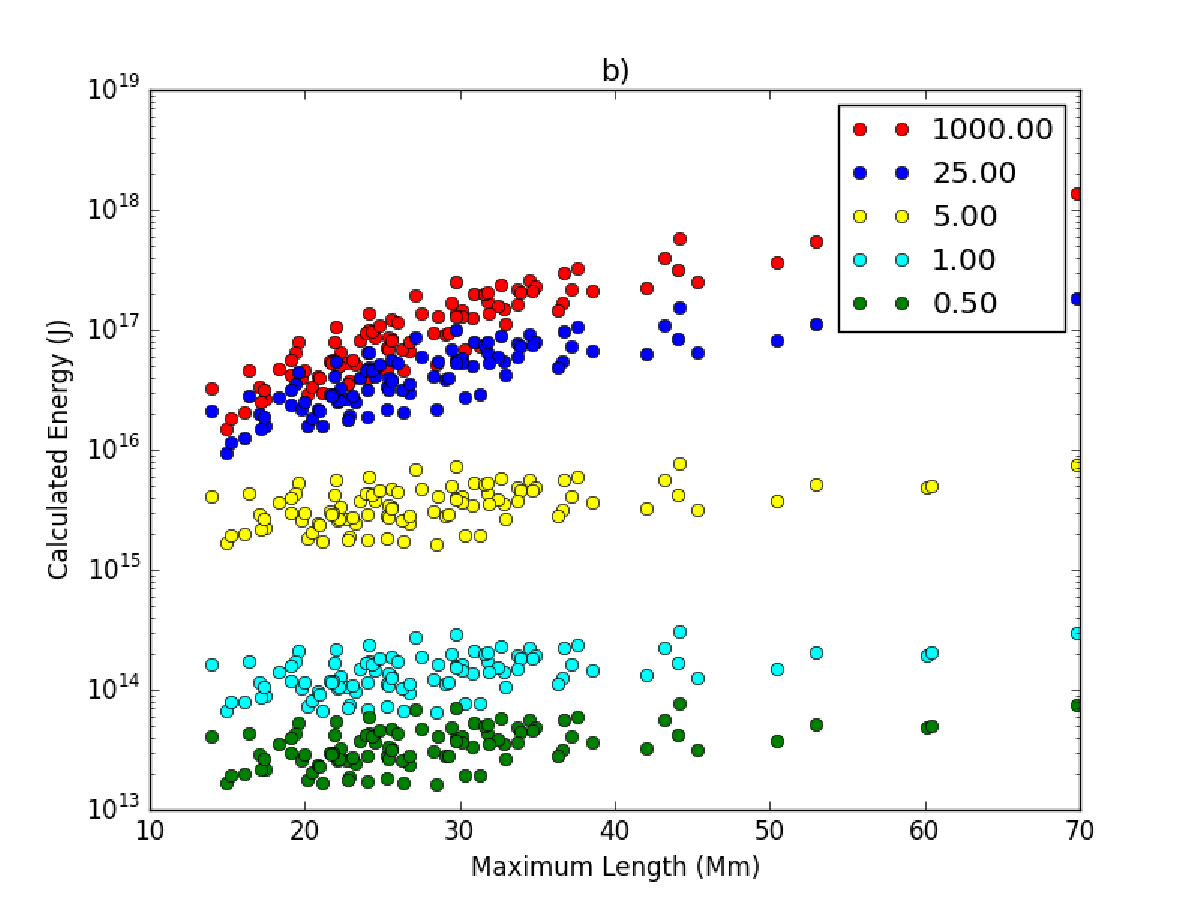
\includegraphics[width=0.48\textwidth]{Chapter3/Figs/scale_h.pdf}
	\caption{\small a) Here we have used two different $\rho_0$ values. Red indicates $\rho_0 = 1.0 \times 10^{-8}\ \textrm{kg/m}^{3}$ and blue indicates $\rho_0 = 1.0 \times 10^{-11}\ \textrm{kg/m}^{3}$. b) The energy required to form a macrospicule plotted as a function of the maximum length of the macrospicule. The maximum length is plotted against the energy required to move a mass to this height. The scale-height value of $1000\ \textrm{Mm}$ here is used as a proxy for uniform density as this is approximately $10$ times greater than the largest macrospicule in the sample, which, makes the assumption valid.}
	\label{fig:scale_h}
\end{figure}

\subsection{Energetics and scale-height}
Examining the energy required to generate MS is a worthwhile task, in reference to the process to which they are formed. At the limb $g = 276\ \textrm{ms}^2$, hence, the gravitational scale-height will need to be taken into account when performing any calculations. \cite{Pereira2012} has studied this behaviour in the case of spicules, however, no such study has been performed for MS to date. We have modelled the MS simply as a column of plasma, with no magnetic field influences, and considered the potential energy required to reach the height at which they are observed. Choosing a $\rho_0$ is important, measurements by \cite{Parenti2002} and \cite{Withbroe1976} give densities of MS as $1.0 \times 10^{-11}$ kg/m$^{3}$. However, we assume here a scale-height over the extension of the macrospicule and these authors measure the `body' of the macrospicule. As such, we use a $\rho_0$ taken from \cite{Vernazza1981}, $\rho_0 = 1.0 \times 10^{-8}\ \textrm{kg/m}^{3}$. Given that we use a scale-height and applying our $\rho_0$ at the footpoint, we will obtain a sensible value for the energy required to form a macrospicule.

The centre of mass was estimated, and the potential energy necessary to move the mass from the limb this point defined as:

\begin{equation}
R_y = \frac{Le^{-L/H} - He^{-L/H} + H}{1 + e^{-L/H}},
\end{equation} 

\noindent where $R_y$ is the distance from the solar limb, $H$ is the scale-height and $L$ is the maximum length of the macrospicule.

Integrating over the volume of the macrospicule, taking into account the scale-height, estimated the mass. Applying the mass as a point at $R_y$, the minimum mechanical energy required to form a macrospicule is equal to the potential energy at $R_y$. \cref{fig:scale_h} demonstrates how the estimated energy required will change dependent on the scale-height of the plasma contained within the macrospicule.

As is intuitive, the more uniform the density, the higher the energy required to form the macrospicule. Noticeable are the gradients at higher scale-heights, $1.61 \times 10^{16}\ \textrm{J/Mm}$ with uniform scale-height, and, when $H = 0.5\ \textrm{Mm}$ the gradient is  $6.88 \times 10^{11}\ \textrm{J/Mm}$. This is important as the more energy required to form a macrospicule of a given length, the less likely they are to form. Instances of MS in uniform density and with a scale-height of $25$ Mm are similar below heights of $25\ \textrm{Mm}$.

Macrospicules have been proposed as a source of coronal heating. In order to estimate how much mechanical energy could potentially be transferred from the MS into the corona, we will assume that at any given moment, a macrospicule is occurring at the limb. Assuming that measurements taken here are within $\pm10\ \textrm{Mm}$ of the plane of sky, we take the next interval in which a macrospicule occurs as the angular distance, covering the $\pm10\ \textrm{Mm}$ over the plane of sky, starting at the boundary of the previous interval. 

Extrapolating this around the rest of the solar surface and applying the mean macrospicule count per two hour sample, $1.9$, to each interval a power output can be estimated. Assuming further that all mechanical energy is transferred from the macrospicule into the corona, the power output for uniform scale-height MS is calculated to be $0.153 \times 10^{-3}\ \textrm{W/m{2}}$ and decreasing with the scale-height. Given the power requirements for coronal heating in \cite{AschwandenCHR2007}, MS are an unlikely source for major coronal heating.


\section{Conclusion}
\label{sec:conc1}
Now, let us summarise the general properties for the population of MS (see \cref{table:final-properties}). In general, the values presented here fall between those presented in \cite{Bohlin1975} and \cite{Dere89}. The more extreme examples, seen in \cite{Bohlin1975}, are not found here. We find that the data in \cite{Dere89} are conservative and we find maximum length and lifetimes which are larger. 


\begin{sidewaystable}[t!]
	\centering
	\begin{tabular}{c c c c}
		\hline\hline
		Study & \cite{Bohlin1975} & \cite{Dere89} & The present study \\    
		\hline                                
		Max Length [Mm] & $5.8$-$43.5$ & $1.45$-$16.7$ $\bar{x}$:$8.7$ & $14.0$-$60.4$ $\bar{x}$:$28.1$ \\
		Width [Mm] & $3.6$-$10.9$ & $2.2$-$6.5$ $\bar{x}$:$4.4$ & $3.1$-$16.1$ $\bar{x}$:$7.6$ \\
		Lifetime [min] & $8$-$45$ & $> 3$ & $2.7$-$28.1$ $\bar{x}$:$13.6$ \\
		Max Velocity [km/s] & $10$-$150$ & $20$-$50$ & $54.1$-$105.6$ $\bar{x}$:$109.7$ \\
		Count & $25$ & $10$ & $101$ \\
		Cadence [s] & > $180$ & $20$,$60$ & $12$ \\
		\hline 
	\end{tabular}
	\caption{General properties table. Comparing the values given by \cite{Bohlin1975}, \cite{Dere89} and this study.}
	\bigskip\bigskip

	\begin{tabular}{|c|c|c|c|c|c|c|c|c|c|c|c|c|}
				\hline 
				Magnetic Configuration & \multicolumn{3}{c|}{Velocity (km/s)} & \multicolumn{3}{c|}{Length (Mm)} & \multicolumn{3}{c|}{Width (Mm)} & \multicolumn{3}{c|}{Lifetime (min)}\tabularnewline
				\hline 
				\hline 
				& \multicolumn{1}{c|}{Low} & High & Mean & Low & High & Mean & \multicolumn{1}{c|}{Low} & High & Mean & Low & High & Mean\tabularnewline
				\hline 
				Coronal Hole & 58.3 & 181.3 & 113.4 & 17.3 & 60.4 & 31.9 & 3.1 & 13.0 & 7.2 & 7.8 & 28.6 & 13.5\tabularnewline
				\hline 
				Coronal Hole Boundary & 66.8 & 194.8 & 107.4 & 16.1 & 60.4 & 30.5 & 4.0 & 16.1 & 7.9 & 9.8 & 22.0 & 14.0\tabularnewline
				\hline 
				Quiet Sun & 62.8 & 154.3 & 101.2 & 14.0 & 45.3 & 25.6 & 3.4 & 12.6 & 7.8 & 5.6 & 24.0 & 13.5\tabularnewline
				\hline 
	\end{tabular}
	\caption{Properties associated with each region of the solar limb.}
	\label{table:final-properties}
	
\end{sidewaystable}


Examining the individual regions, in which the MS occur, it is evident that higher velocities are found in the coronal hole and coronal hole boundaries and so we consider the question of whether there might be a difference in the physics of formation to that in the quiet Sun. Examining the lengths, the coronal hole/boundary MS are longer than those seen in the quiet Sun. Open magnetic field lines in coronal holes are the likely cause allowing the MS to extend higher in these regions. We find little difference in the widths, and, examining mean lifetime values, we find percentage differences from the total sample mean: $3.7\%$ and $2.6\%$ for quiet Sun and coronal hole boundary respectively, with a small increase in percentage difference of $-5.3\%$ for coronal hole MS.

Upon examining the general properties and their relations to each other, we also find that the maximum velocity and maximum length are related, and, that the lifetime and maximum length show signs of correlation. However, the maximum velocity and lifetime appear to show little correlation with the current sample size.

A range of magnetic environments have been shown to yield MS with different basic properties in some cases. This may be due to separate generation processes, although this is just a conjecture. The overlying solar environment is more likely to have an effect, either restricting or allowing extension, which would explain the comparatively longer MS observed in coronal holes.

Considering the change of the properties over the sample time period, we find that the maximum length and lifetimes both show a general correlation with the sample time period. Whereas, the maximum velocity does not follow the same pattern, which is somewhat unexpected due to the maximum length being related to the maximum velocity. Consequently, one might expect the maximum velocity to increase as a function of the sample time period. At present we cannot offer any explanation as to why this is the case, but further modelling studies will hopefully reveal some answers.

We observe similar durations for regression back to the limb for the estimates and the recorded times. 
Clearly, there is a greater variance in the measured values compared to the estimates, but this is to be expected.
The mean time for the tip to recede back to the limb is $7.5\ \textrm{min}$ (estimated) and $6.6\ \textrm{min}$ (recorded), which are similar, indicating that gravity is the dominating force behind their fall. 
This small difference between reading and model is not large enough to be significant, or draw any conclusions.

Lastly, let us estimate the energy required to generate the MS. We incorporated the scale-height variations over the length of the macrospicule, such that, the density decreases from footpoint to tip. This was applied to take into account non-uniform density when estimating the centre of mass. 
We find that high scale-heights yield high energy requirements, which decrease with lower value scale-heights.
Examining the mean macrospicule energy values for the scale-heights we obtain $1.46 \times 10^{17}\ \textrm{J}$, $4.78 \times 10^{16}\ \textrm{J}$,  $3.09 \times 10^{15}\ \textrm{J}$, $1.46 \times 10^{14}\ \textrm{J}$ and $3.66 \times 10^{13}\ \textrm{J}$ for scale-heights of uniform and $25, 5, 1$ and $0.5\ \textrm{Mm}$, respectively.

Our simple energetics model yields values for energy which are possibly too small, bit are still realistic. If we compare these to energies calculated for wave-driven reconnection events in \cite{Heggland2009}, of the order $10^{17}$-$10^{18}\ \textrm{J}$ , if the scale-height is around 10-25 Mm according to our estimates, the generation of MS may be feasible. However, this model generates jets of $1$ Mm in length, a degree of magnitude away from our measurements. Models have been proposed, such as \cite{Adams2014}, in which open magnetic field above a reconnection event allows the MS to extend to the heights we observe.

It would be preferable to have $8$-$10$ years worth of high-quality data to examine the possible changes in the properties of MS over the solar cycle. Also, investigating the rotational speed of MS, which is not possible without spectral information, would be feasible and would give additional insight. The use of modelling to understand these features further would also be of interest such that we might be able to understand how these features are generated.  



\begin{pycode}[chapter3]
ch3 = texfigure.Manager(pytex, number=2, base_path='./Chapter3/')
\end{pycode}
